%
\documentclass[10pt,a4paper]{article}


\usepackage{array}
\usepackage{subfigure}
\usepackage{graphicx}
\usepackage{amssymb}
\usepackage{amsmath}
\usepackage{cite}
\usepackage{color}
\usepackage{url}
\usepackage[lined,linesnumbered,ruled,norelsize]{algorithm2e}
\usepackage{listings}
\lstset{
  language=Octave, 
  basicstyle=\footnotesize, 
  frame=single, 
  showspaces=false, 
  showstringspaces=false}


\begin{document}

\title{Experiment 1: Linear Regression}

\maketitle
  
\section{Description}
%
  This first exercise will give you practice with linear regression. These exercises have been extensively tested with Matlab, but they should also work in Octave, which has been called a ``free version of Matlab''. If you are using Octave, be sure to install the Image package as well (available for Windows as an option in the installer, and available for Linux from Octave-Forge ).


\section{Linear Regression}
%
  Recall that the linear regression model is 
  %
  \begin{equation}
    h_{\theta}(x) = \theta^Tx = \sum_{j=0}^n \theta_j x_j,
  \label{eq:lrmodel}
  \end{equation}
  %
  where $\theta$ is the parameter which we need to optimize and $x$ is the $(n+1)$-dimensional feature vector \footnote{A training data is actually $n$-dimensional, i.e., $x = [x_1, x_2, \cdots, x_n]$. For each training data, we have an extra intercept item $x_0 = 1$. Therefore, the resulting feature vector is $(n+1)$-dimensional.}. Given a training set $\{x^{(i)}\}_{i=1,\cdots,m}$, our goal is to find the optimal value of $\theta$ such that the objective function $J(\theta)$, as shown in Equation (\ref{eq:lrobj}), can be minimized. 
  %
  %
  \begin{equation}
    J(\theta) = \frac{1}{2m}\sum^m_{i=1} (h_\theta(x^{(i)}) - y^{(i)})^2
  \label{eq:lrobj}
  \end{equation}
  %
  %
  One of the optimization approach is gradient descent algorithm. The algorithm is performed iteratively, and in each iteration, we update parameter $\theta$ according to the the following rule
  %
  \begin{equation}
    \theta_j := \theta_j - \alpha \frac{1}{m} \sum_{i=1}^m (h_\theta(x^{(i)}) - y^{(i)}) x^{(i)}_j 
  \end{equation}
  %
  where $\alpha$ is so-called ``learning rate'' based on which we can tune the convergence of the gradient descent.
  %




\section{2D Linear Regression} \label{sec:2dlr}
%
  We start a very simple case where $n=1$. Download data1.zip, and extract the files (ex1x.dat and ex1y.dat) from the zip file. The files contain some example measurements of heights for various boys between the ages of two and eights. The y-values are the heights measured in meters, and the x-values are the ages of the boys corresponding to the heights. Each height and age tuple constitutes one training example  $(x^{(i)}, y^{(i)}$ in our dataset. There are $m = 50$ training examples, and you will use them to develop a linear regression model using gradient descent algorithm, based on which, we can predict the height given a new age value.

  In Matlab/Octave, you can load the training set using the commands
  %
  %
  \begin{lstlisting}
    x = load('ex1x.dat');
    y = load('ex1y.dat');
  \end{lstlisting}
  %
  This will be our training set for a supervised learning problem with $n=1$ features ( in addition to the usual  $x_0 = 1$, so  $x \in {\mathbb R}^2$ ). If you're using Matlab/Octave, run the following commands to plot your training set (and label the axes):
  %
  %
  \begin{lstlisting}
    figure % open a new figure window
    plot(x, y, 'o');
    ylabel('Height in meters')
    xlabel('Age in years')
  \end{lstlisting}
  %
  You should see a series of data points similar to Fig.~\ref{fig:data}.
  %
  \begin{figure}[h!]
    \centering
      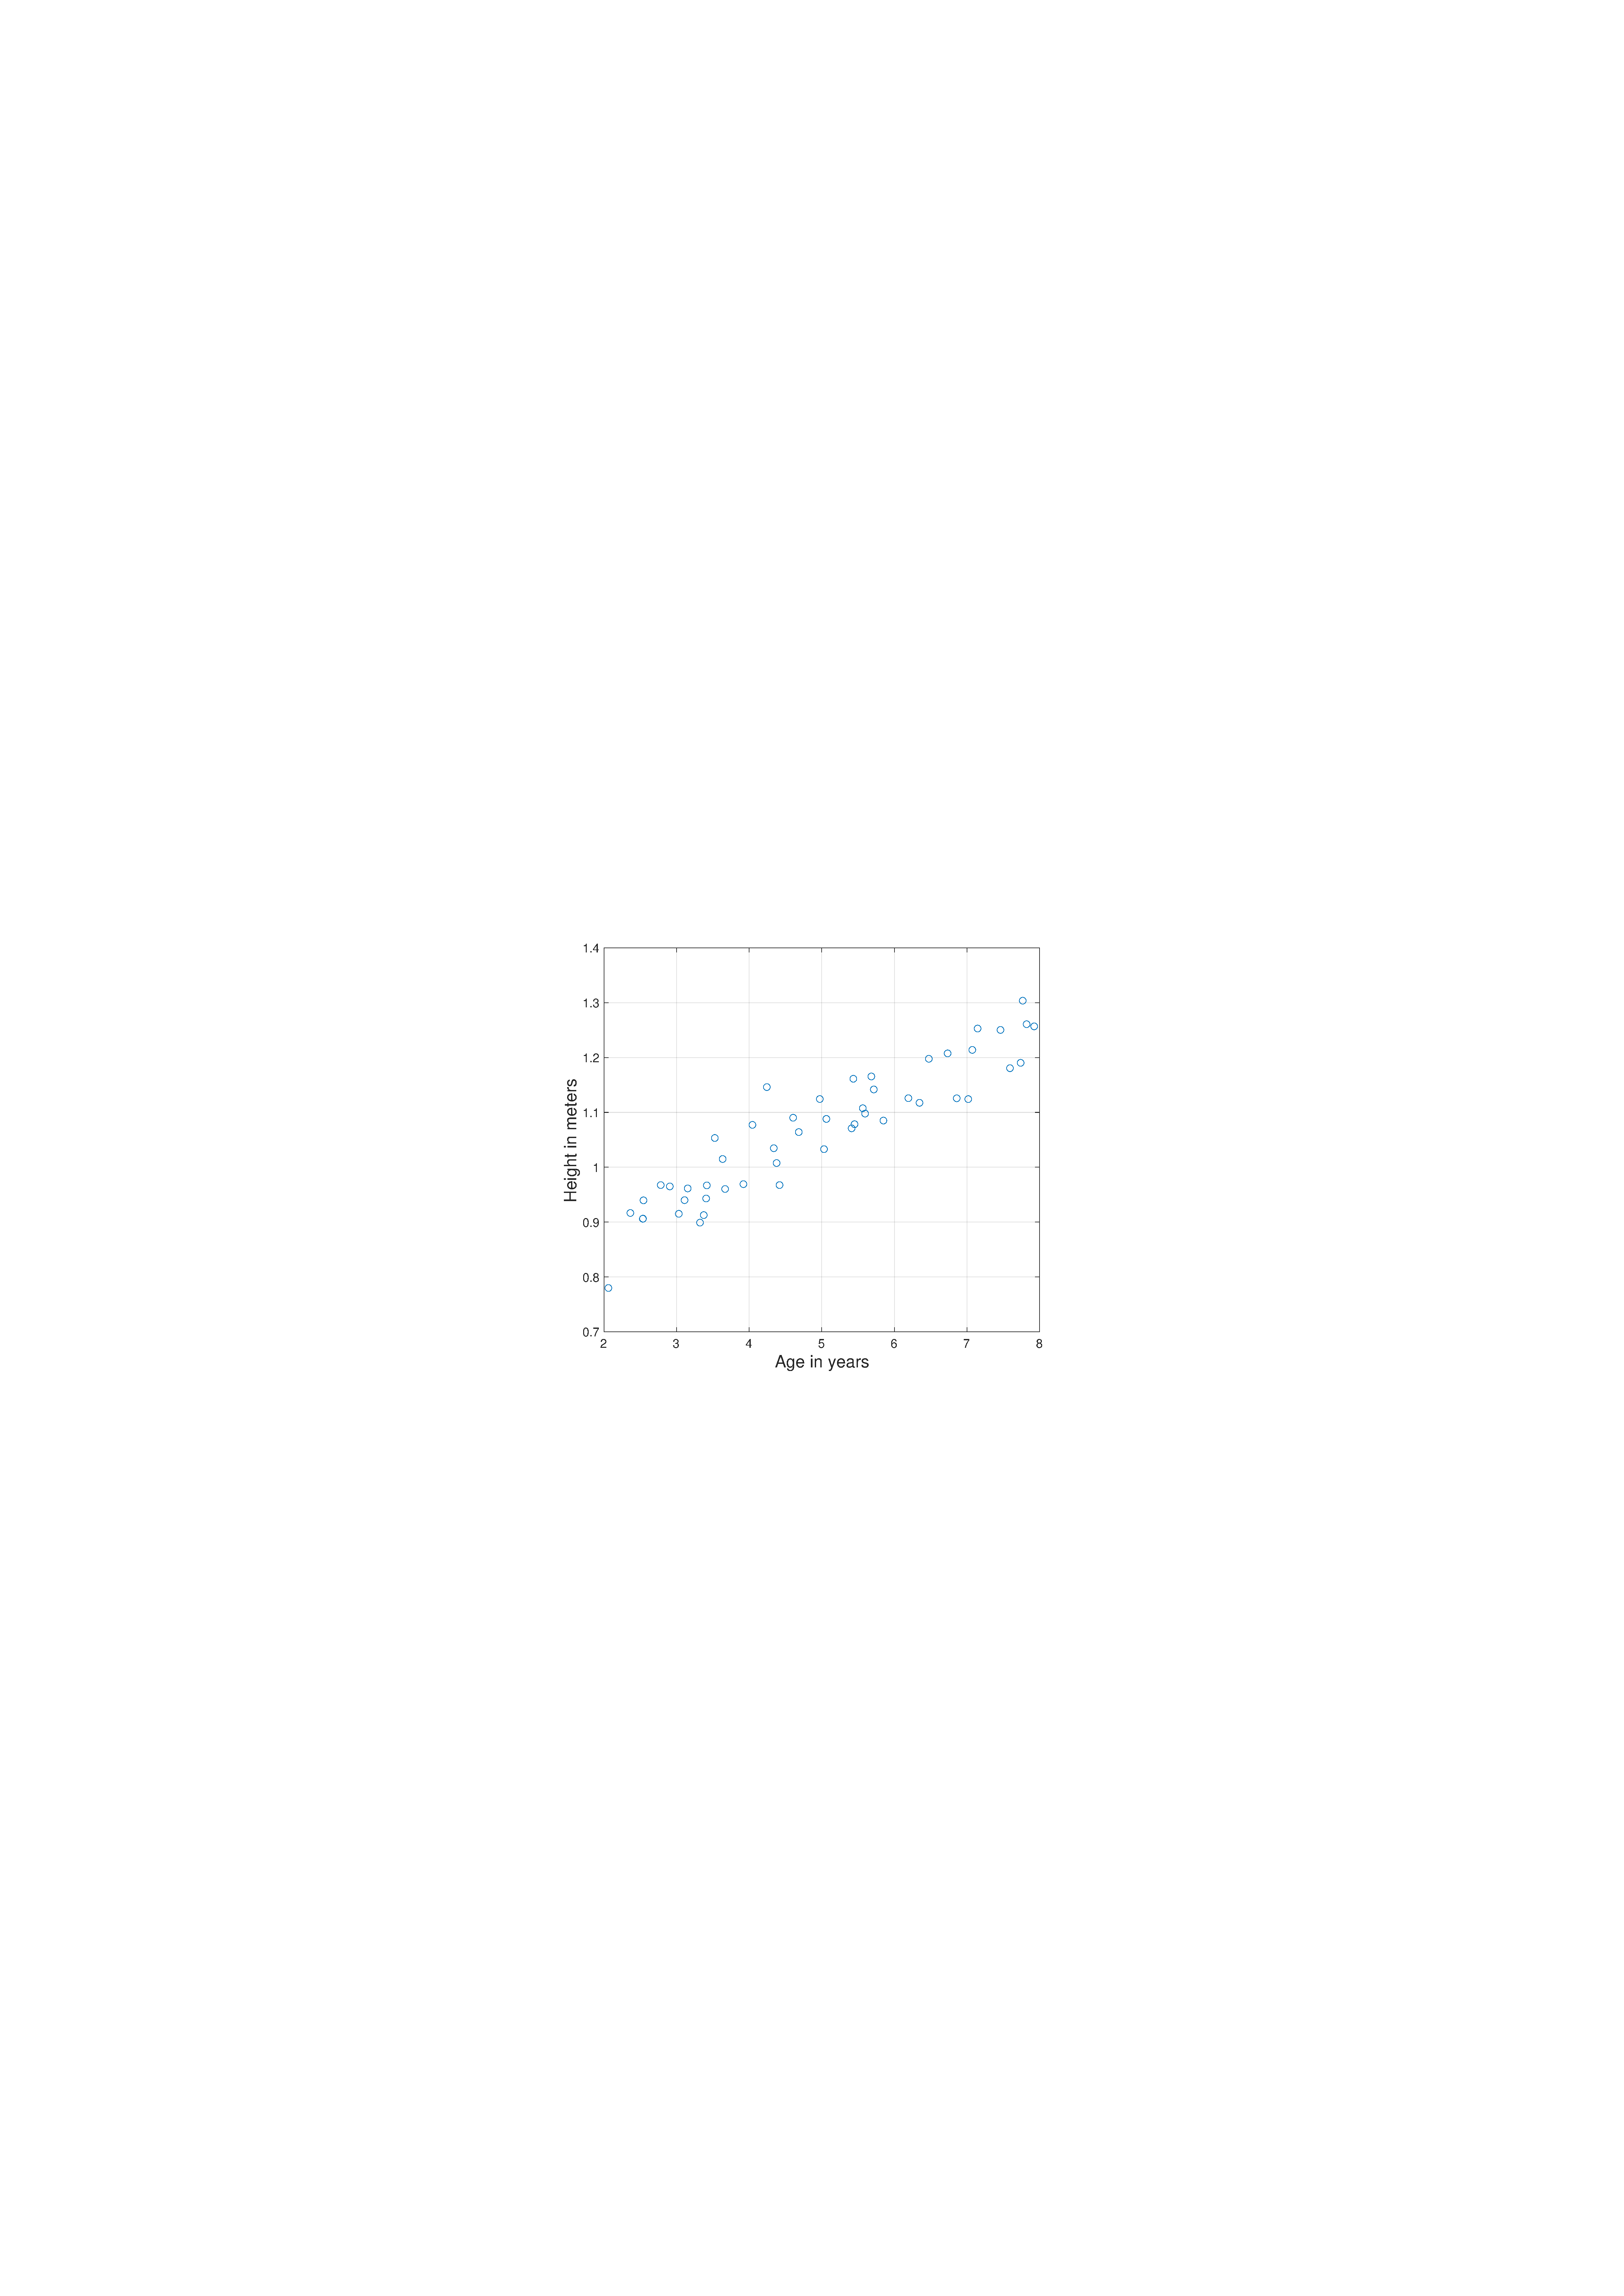
\includegraphics[width=.7\columnwidth]{datasample}
      \caption{Plotting the data.}
      \label{fig:data}
  \end{figure}

  Before starting gradient descent, we need to add the $x_0 = 1$ intercept term to every example. To do this in Matlab/Octave, the command is
  %
  \begin{lstlisting}
    m = length(y); % store the number of training examples
    x = [ones(m, 1), x]; % Add a column of ones to x
  \end{lstlisting}
  %
  From this point on, you will need to remember that the age values from your training data are actually in the second column of x. This will be important when plotting your results later.


  We implement linear regression for this problem. The linear regression model in this case is
  %
  %
  \begin{equation}
    h_{\theta}(x) = \theta^T x = \sum_{i=0}^1 \theta_i x_i = \theta_1 x_1 + \theta_2,
  \end{equation}
  %

  \noindent\textbf{(1)} Implement gradient descent using a learning rate of $\alpha = 0.07$. Initialize the parameters to  $\theta = \vec{0}$ (i.e.,  $\theta_0=\theta_1=0$), and run one iteration of gradient descent from this initial starting point. \textbf{Record the value of of $\theta_0$ and $\theta_1$ that you get after this first iteration.} 


  \vspace{2ex}
  \noindent\textbf{(2)} Continue running gradient descent for more iterations until $\theta$ converges. (this will take a total of about 1500 iterations). \textbf{After convergence, record the final values of $\theta_0$ and $\theta_1$ that you get, and plot the straight line fit from your algorithm on the same graph as your training data according to $\theta$.} The plotting commands will look something like this:
  %
  \begin{lstlisting}
    hold on % Plot new data without clearing old plot
    plot(x(:,2), x*theta, '-') % remember that x is now a matrix
                               % with 2 columnsand the second 
                               % column contains the time info
    legend('Training data', 'Linear regression')

  \end{lstlisting}
  %
  Note that for most machine learning problems, $x$ is very high dimensional, so we don't be able to plot $h_\theta(x)$. But since in this example we have only one feature, being able to plot this gives a nice sanity-check on our result.

  \vspace{2ex}
  \noindent\textbf{(3)} Finally, we'd like to make some predictions using the learned hypothesis. \textbf{Use your model to predict the height for two boys of ages 3.5 and 7.}



  


\section{Understanding $J(\theta)$}
%
  We'd like to understand better what gradient descent has done, and visualize the relationship between the parameters  $\theta \in {\mathbb R}^2$ and $J(\theta)$. In this problem, we'll plot $J(\theta)$ as a 3D surface plot. (When applying learning algorithms, we don't usually try to plot $J(\theta)$ since usually  $\theta \in {\mathbb R}^n$ is very high-dimensional so that we don't have any simple way to plot or visualize $J(\theta)$. But because the example here uses a very low dimensional  $\theta \in {\mathbb R}^2$, we'll plot $J(\theta)$ to gain more intuition about linear regression.)

  %
  \begin{figure}[htb!]
    \centering
      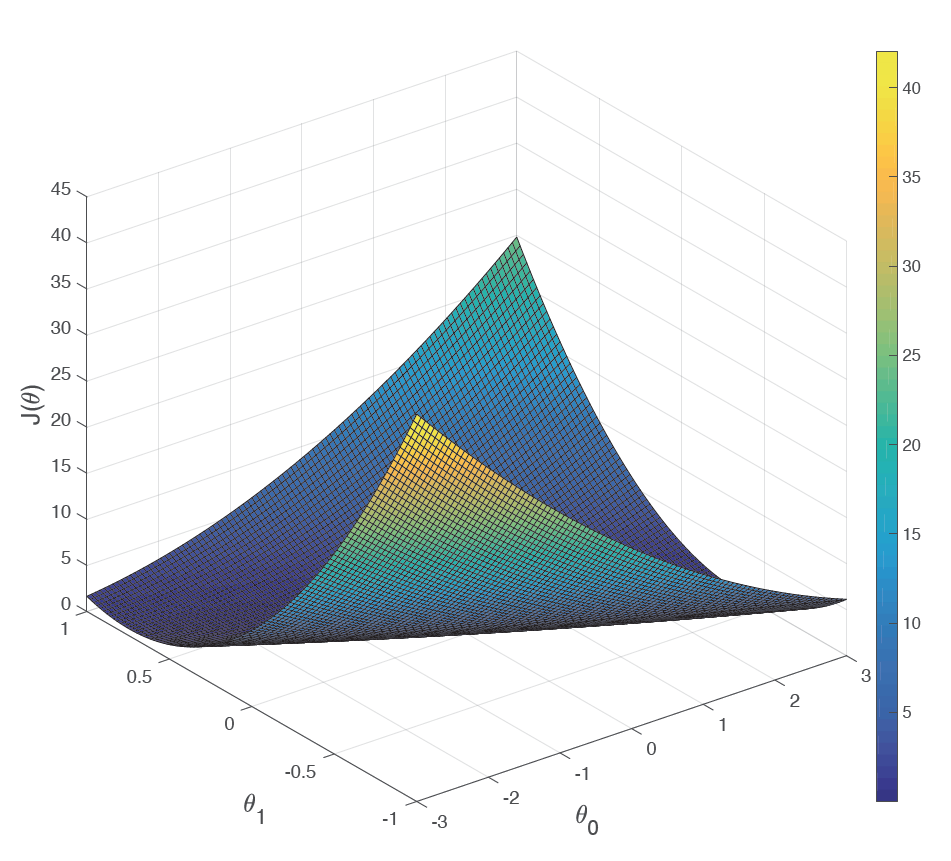
\includegraphics[width=.6\columnwidth]{surface.png}
      \caption{The relationship between $J$ and $\theta$}
      \label{fig:surf}
  \end{figure}

  To get the best viewing results on your surface plot, use the range of theta values that we suggest in the code skeleton below.
  %
  %
  \begin{lstlisting}
    J_vals = zeros(100, 100); % initialize Jvals to
                              % 100*100 matrix of 0's
    theta0_vals = linspace(-3, 3, 100);
    theta1_vals = linspace(-1, 1, 100);
    for i = 1:length(theta0_vals)
        for j = 1:length(theta1_vals)
        t = [theta0_vals(i); theta1_vals(j)];
        J_vals(i,j) = %% YOUR CODE HERE %%
        end
    end

    % Plot the surface plot
    % Because of the way meshgrids work in the surf command, we 
    % need to transpose J_vals before calling surf, or else the 
    % axes will be flipped
    J_vals = J_vals'
    figure;
    surf(theta0_vals, theta1_vals, J_vals)
    xlabel('\theta_0'); ylabel('\theta_1')
  \end{lstlisting}
  %
  You should get a figure similar to Fig.~\ref{fig:surf}. If you are using Matlab/Octave, you can use the orbit tool to view this plot from different viewpoints.
  

  \textbf{What is the relationship between this 3D surface and the value of $\theta_0$ and $\theta_1$ that your implementation of gradient descent had found? Visualize the relationship by both \emph{surf} and \emph{contour} commands.}

  \vspace{2ex}
  \noindent\emph{Remarks}: For the \textsf{surf} function \textsf{surf(x, y, z)}, if $x$ and $y$ are vectors, $x = 1:columns(z)$ and $y=1:rows(z)$. Therefore, $z(i, j)$ is actually calculated based on $x(j)$ and $y(i)$. This rule is also applicable to the contour function. We can specify the number and the distribution of contours in the \textsf{contour} function, by introduction different spaced vector, e.g., linearly spaced vector (\textsf{linspace}) and logarithmically spaced vector (\textsf{logspace}). Try both in this exercises and select the better one to improve the illustration. 



\section{Multivariate Linear Regression}
%
  We now look at a more complicated case where each training data contains multiple features. Download data1.zip, and extract the files (ex2x.dat and ex2y.dat) from the zip file. This is a training set of housing prices in Portland, Oregon, where the outputs $y$'s are the prices and the inputs $x$'s are the living area and the number of bedrooms. There are $m=47$ training examples.

  Take a look at the values of the inputs $x^{(i)}$ and note that the living areas are about 1000 times the number of bedrooms. This difference means that preprocessing the inputs will significantly increase gradient descent's efficiency.

  In your program, scale both types of inputs by their standard deviations and set their means to zero. In Matlab/Octave, this can be executed with
  %
  \begin{lstlisting}[language=Octave, basicstyle=\footnotesize, showspaces=false]
    sigma = std(x);
    mu = mean(x);
    x(:,2) = (x(:,2) - mu(2))./ sigma(2);
    x(:,3) = (x(:,3) - mu(3))./ sigma(3);
  \end{lstlisting}


\subsection{Selecting A Learning Rate Using $J(\theta)$}
%
  Now it's time to select a learning rate $\alpha.$ The goal of this part is to pick a good learning rate in the range of 
  %
  \[ 0.001 \leq \alpha \leq 10 \]
  %
  You will do this by making an initial selection, running gradient descent and observing the cost function, and adjusting the learning rate accordingly. Recall that the cost function is defined in Equation~(\ref{eq:lrobj}). The cost function can also be written in the following vectorized form,
  %
  \begin{displaymath}
    J(\theta) = \frac{1}{2m}\left(X\theta-\vec{y}\right)^{T}(X\theta-\vec{y}) \nonumber
  \end{displaymath}  
  %
  where
  %
  \[
    \vec y = \begin{bmatrix}
      y^{(1)} \\
      y^{(2)} \\
      \vdots \\
      y^{(m)}
      \end{bmatrix}, \hspace{3ex}
    %
    X = \begin{bmatrix}
      -(x^{(1)})^T- \\
      -(x^{(2)})^T- \\
      \vdots \\
      -(x^{(m)})^T-
      \end{bmatrix}
  \]
  % \begin{figure}[htb!]
  %   \centering
  %     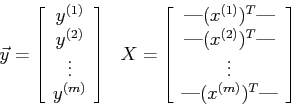
\includegraphics[width=.5\columnwidth]{img2-1}
  % \end{figure}
  %
  The vectorized version is useful and efficient when you're working with numerical computing tools like Matlab/Octave. If you are familiar with matrices, you can prove to yourself that the two forms are equivalent.

  While in the previous exercise you calculated $J(\theta)$ over a grid of $\theta_0$ and $\theta_1$ values, you will now calculate $J(\theta)$ using the $\theta$ of the current stage of gradient descent. After stepping through many stages, you will see how $J(\theta)$ changes as the iterations advance.

  Now, run gradient descent for about 50 iterations at your initial learning rate. In each iteration, calculate $J(\theta)$ and store the result in a vector $J$. After the last iteration, plot the $J$ values against the number of the iteration. In Matlab/Octave, the steps would look something like this:
  %
  \begin{lstlisting}[language=Octave, basicstyle=\footnotesize, showspaces=false]
    theta = zeros(size(x(1,:)))'; % initialize fitting parameters
    alpha = %% Your initial learning rate %%
    J = zeros(50, 1); 

    for num_iterations = 1:50
      J(num_iterations) = %% Calculate your cost function here %%
      theta = %% Result of gradient descent update %%
    end

    % now plot J
    % technically, the first J starts at the zero-eth iteration
    % but Matlab/Octave doesn't have a zero index
    figure;
    plot(0:49, J(1:50), '-')
    xlabel('Number of iterations')
    ylabel('Cost J')
  \end{lstlisting}
  %
  If you picked a learning rate within a good range, your plot should appear like the figure below.
  %
  \begin{figure}[htb!]
    \centering
      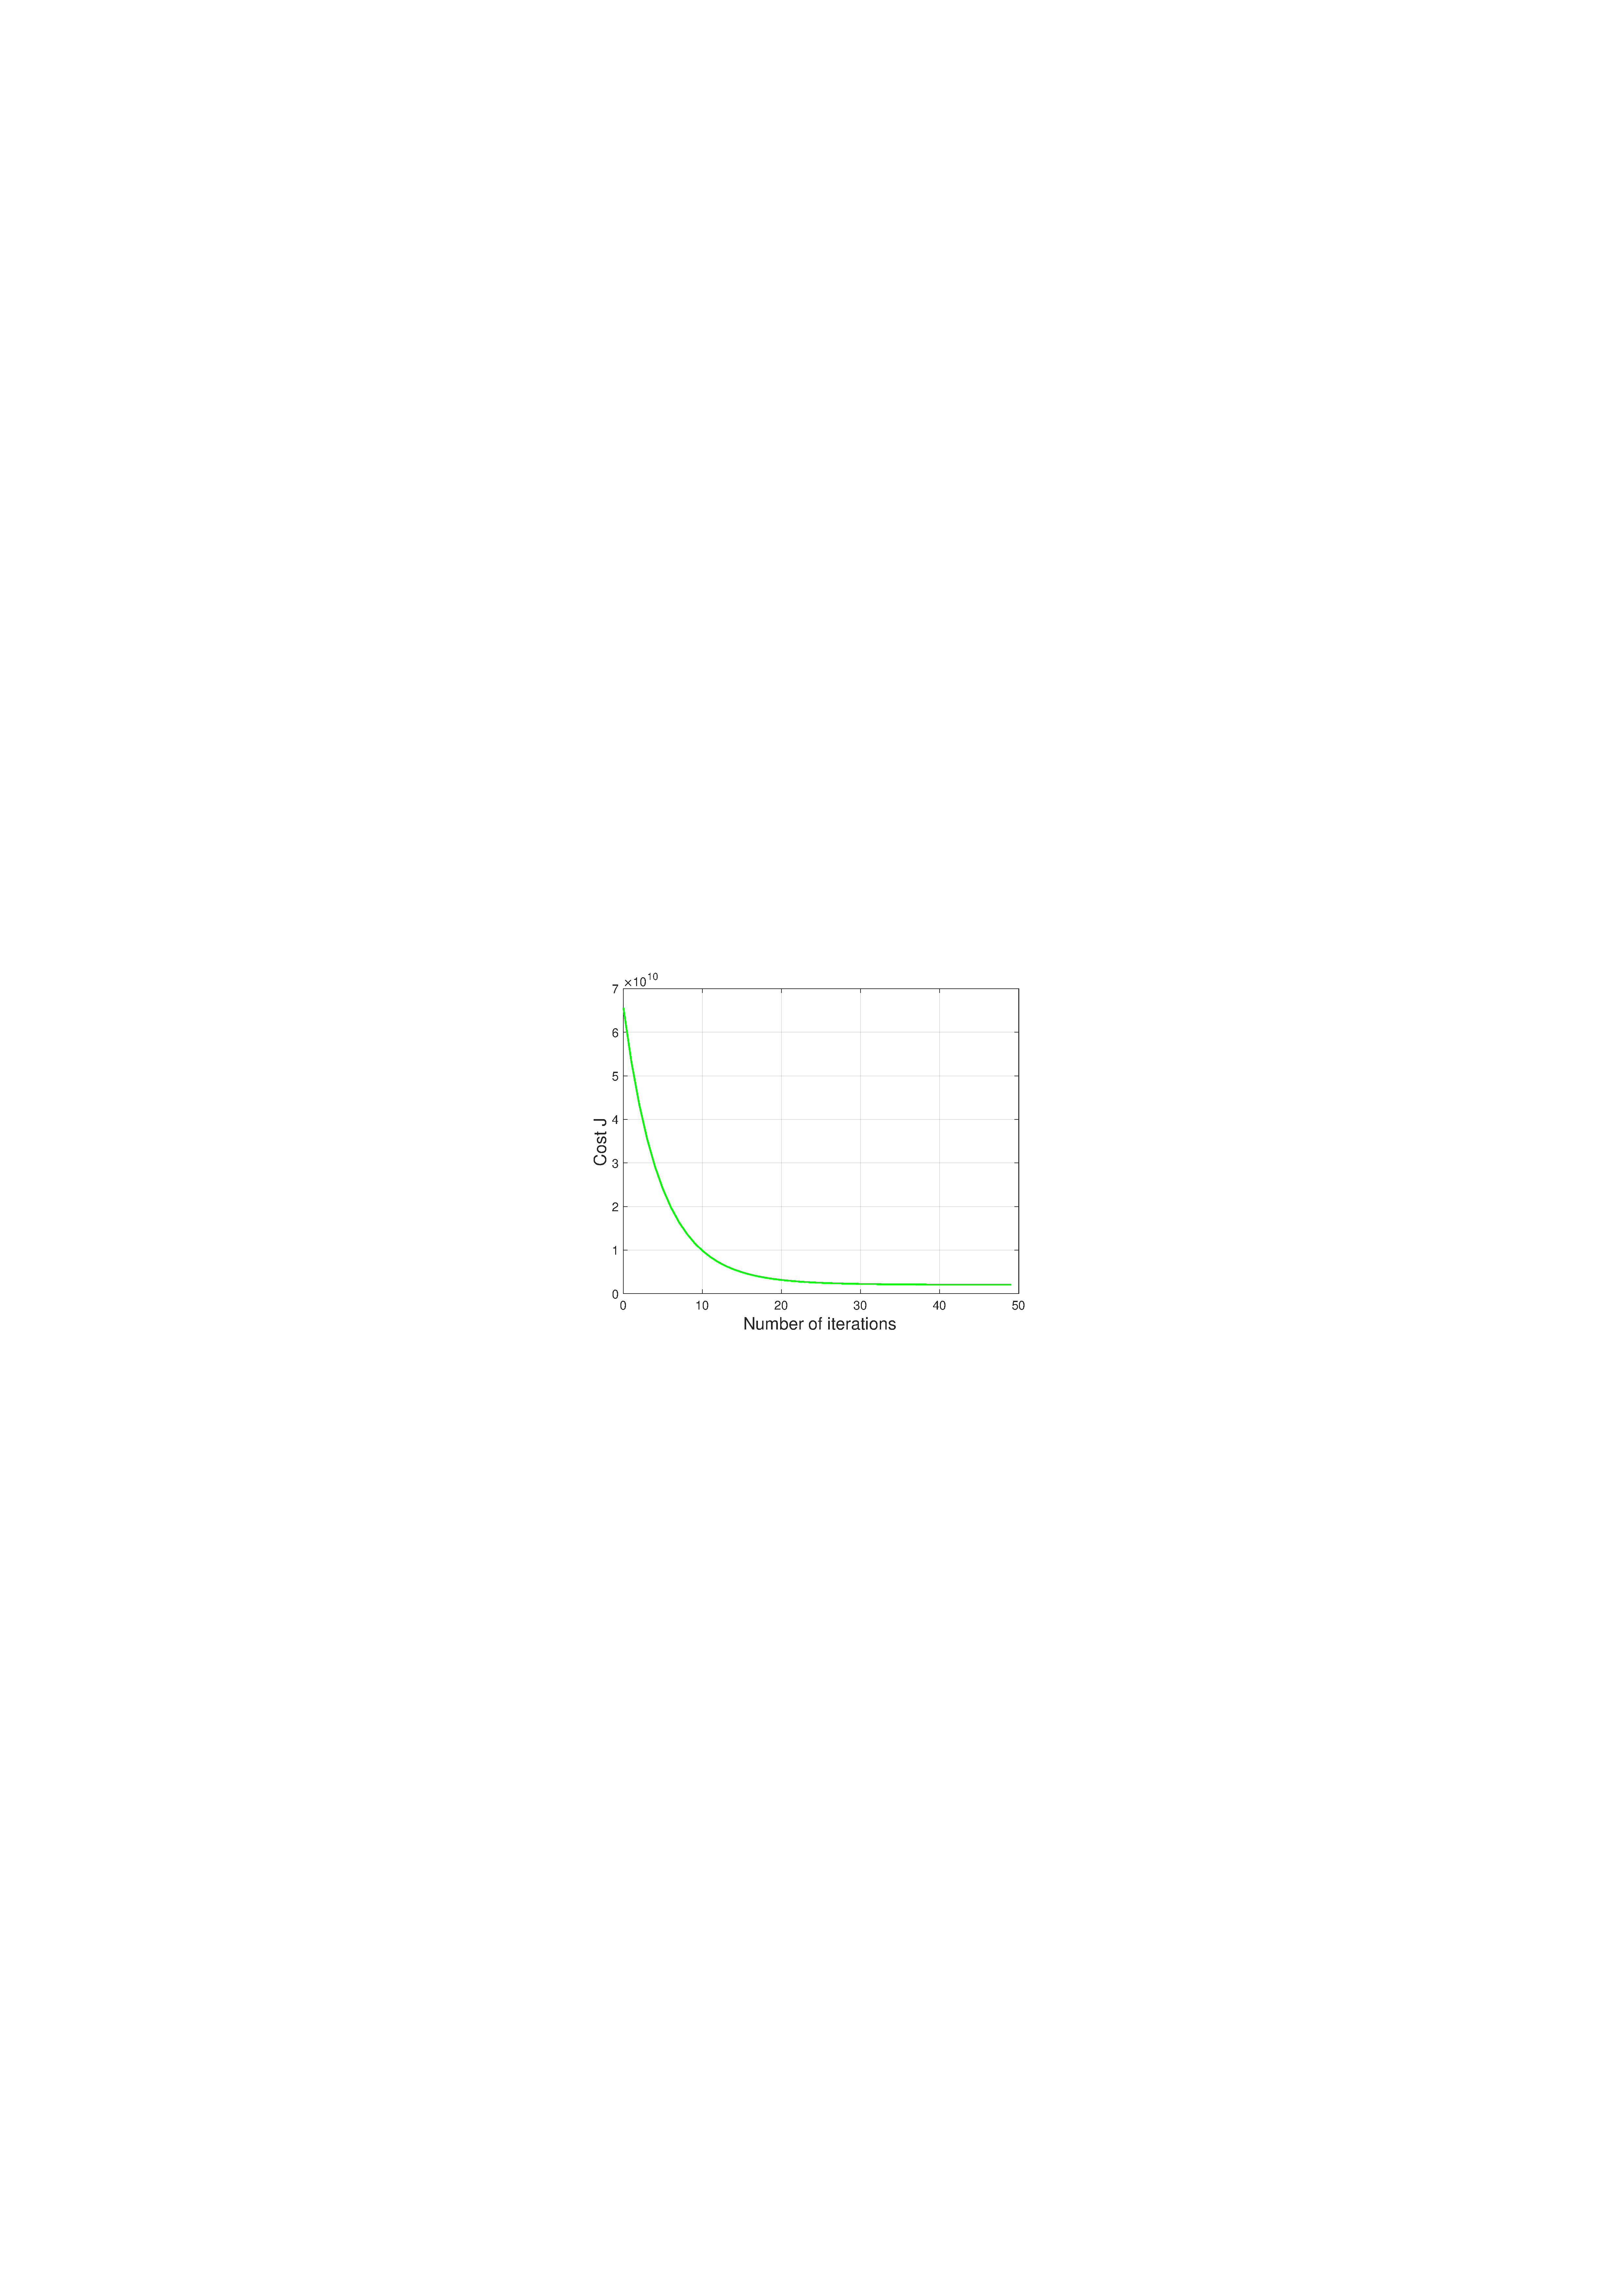
\includegraphics[width=.7\columnwidth]{lrate}
  \end{figure}


  If your graph looks very different, especially if your value of $J(\theta)$ increases or even blows up, adjust your learning rate and try again. We recommend testing alphas at a rate of of 3 times the next smallest value (i.e. 0.01, 0.03, 0.1, 0.3 and so on). You may also want to adjust the number of iterations you are running if that will help you see the overall trend in the curve.

  To compare how different learning learning rates affect convergence, it's helpful to plot J for several learning rates on the same graph. In Matlab/Octave, this can be done by performing gradient descent multiple times with a \textit{hold on} command between plots. Concretely, if you've tried three different values of alpha (you should probably try more values than this) and stored the costs in $J1$, $J2$ and $J3$, you can use the following commands to plot them on the same figure:
  %
  \begin{lstlisting}[language=Octave, basicstyle=\footnotesize, showspaces=false]
    plot(0:49, J1(1:50), 'b-');
    hold on;
    plot(0:49, J2(1:50), 'r-');
    plot(0:49, J3(1:50), 'k-');
  \end{lstlisting}

  The final arguments `b-', `r-', and 'k-' specify different plot styles for the plots. Type
  %
  \begin{lstlisting}[language=Octave, basicstyle=\footnotesize, showspaces=false]
    help plot
  \end{lstlisting}
  %
  at the Matlab/Octave command line for more information on plot styles.

  \textbf{Answer the following questions:}
  % %
  %
  % Observe the changes in the cost function happens as the learning rate changes. What happens when the learning rate is too small? Too large?
  %
  % Using the best learning rate that you found, run gradient descent until convergence to find
  %
  \begin{enumerate}
    \item Observe the changes in the cost function happens as the learning rate changes. What happens when the learning rate is too small? Too large?
    \item Using the best learning rate that you found, run gradient descent until convergence to find
    %
    \begin{enumerate}
      \item The final values of $\theta$
      \item The predicted price of a house with 1650 square feet and 3 bedrooms. Don't forget to scale your features when you make this prediction!
    \end{enumerate}
  \end{enumerate}







\end{document}
